\documentclass{beamer}

\usepackage{beamerthemesplit}
\usetheme{Singapore} 

\input{../../include/preamble.inc} 
\input{../../include/definitions.inc} 
\input{../../include/author.inc} 

\title[]{Стационарные изоэнтропические течения идеального газа}

\begin{document}
	
\frame[plain]{\titlepage}

\frame[plain]{
	\frametitle{Аннотация}
	\parbox{\textwidth}{
		Уравнение состояния идеального политропного газа. Интеграл Бернулли изоэнтропического течения политропного газа. Параметры торможения потока, максимальная скорость, критическая скорость звука, кри\-ти\-ческая скорость. Формула Сен-Венана--Ванцеля для истечения газа из большого сосуда. Число Маха и коэффициент скорости. Связь параметров торможения и числа Маха и коэффициента скорости. Нагревание тел в потоке газа, влияние сжимаемости на течение.
	}
}

\frame{
	\frametitle{Уравнения состояния идеального политропного газа}
	
	\begin{exampleblock}{Термическое уравнение состояния}
		\parbox{\textwidth}{
			
			\[
			p = p_0 e^{(S-S_0)/c_V} \left( \frac{\rho}{\rho_0} \right)^\gamma = A(S) \rho^\gamma
			\]
			
		}
	\end{exampleblock}

	\begin{exampleblock}{Внутренняя энергия и энтальпия в адиабатном процессе ($S=const$)}
		\parbox{\textwidth}{
			\[ 
				d\varepsilon = T dS  - p d\left( \frac{1}{\rho}\right)  = 
				A(S) \rho^{\gamma-2} d \rho
			\]
			\[
			\Downarrow
			\]
			\[
				\varepsilon = \frac{1}{\gamma-1}\frac{p}{\rho} + \varepsilon_0,\quad
			i = \varepsilon + \frac{p}{\rho} = \frac{\gamma}{\gamma-1}\frac{p}{\rho} + i_0,
			\]
		\medskip
		где $\varepsilon_0$, $i_0$ -- константы интегрирования, которые можно будет опустить.
			
		}
	\end{exampleblock}


	
}

\frame{
	\frametitle{Интеграл Бернулли для изоэнтропического течения политропного газа  }
	
	\begin{exampleblock}{Интеграл Бернулли}
		\parbox{\textwidth}{
			\[
			i^*=\frac{v^2}{2} + \frac{\gamma}{\gamma-1} \frac{p}{\rho} = 
			\frac{v^2}{2} + i = 
			\frac{v^2}{2} + c_p T = 
			C(l), 
			\]
			где $C(l)$ -- константа, характерная для выбранной линии тока; $c_p$ -- коэффициент теплоемкости при постоянном давлении. Массовые силы отсутствуют\footnote{Массовыми силами не всегда можно пренебречь, например, в метеорологии.}.
		}
	\end{exampleblock}

	\begin{exampleblock}{Основные следствия}
		\parbox{\textwidth}{
			\alert{Давление, плотность и температура с ростом скорости вдоль линии тока падают}.
		}
	\end{exampleblock}
	
}

\frame{
	\frametitle{Параметры торможения потока}
	
	\begin{exampleblock}{Температура торможения}
		\parbox{\textwidth}{
			Самая высокая температура на линии тока будет там, где $v = 0$, тогда
			\[
			i^* = c_p T^*,
			\]
			где $T^*$ -- \alert{температура торможения}, а $i^*$ -- \alert{полное теплосодержание}. 
			}
	\end{exampleblock}

	\begin{exampleblock}{Давление и плотность торможения}
		\parbox{\textwidth}{
			\[
			i^* = c_p T^* = 
			\frac{\gamma}{\gamma-1} \frac{p_0^{1/\gamma}}{\rho_0} e^{(S-S_0)/c_p} p^{*(\gamma-1)/\gamma} =
			\]
			\[
			=\frac{\gamma}{\gamma-1} \frac{p_0}{\rho_0^{\gamma}} e^{(S-S_0)/c_p} \rho^{*(\gamma-1)} = 
			\frac{\gamma}{\gamma-1} \frac{p^*}{\rho^*},
			\]
			где $p^*$, $\rho^*$ -- \alert{давление и плотность торможения}.
			
		}
	\end{exampleblock}
	
}

\frame{
	\frametitle{Задача об истечении газа из большого сосуда}
	
	\begin{columns}
		\begin{column}{0.4\textwidth}
			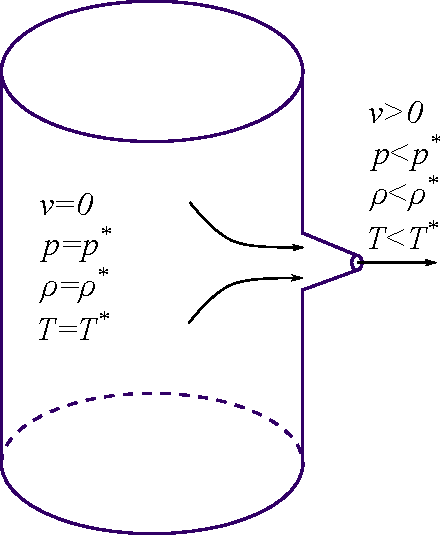
\includegraphics[width=\linewidth]{../img/gasholder.pdf}
		\end{column}
		\begin{column}{0.6\textwidth}
			
			
			\only<1>{
			\parbox{\textwidth}{
				При \alert{установившемся адиабатическом истечении газа} из большого сосуда скорость $v$ в далеких от отверстия точках равна нулю, а давление, плотность и температура соответственно равны давлению торможения, плотности торможения и температуре торможения.
			}}
		
			\only<2>{
				\begin{exampleblock}{Максимальная скорость истечения газа}
					\smallskip
					\parbox{\textwidth}{
						Максимальная скорость \alert{$v_{max}$} достигается при адиабатическом истечении газа в пустоту $p=0$, $\rho=0$, $T=0$:
						\[
						i^* = \frac{v_{max}^2}{2},
						\]
						или
						\[
							v_{max} = \sqrt{2 c_p T^*}.
						\]
					}
				\end{exampleblock}
			}
			
			\only<3>{
				\begin{exampleblock}{Скорость звука}
					\parbox{\textwidth}{
						Для совершенного газа скорость звука имеет вид
						\[
						c = \sqrt{\left(\pd{p}{\rho}\right)_S}=\sqrt{\frac{\gamma p}{\rho} } = \sqrt{\gamma R T}.
						\]
					}
				\end{exampleblock}
			
				\begin{exampleblock}{Интеграл Бернулли}
					\parbox{\textwidth}{
						\[
						\frac{v^2}{2} + \frac{c^2}{\gamma - 1} = \frac{v_{max}^2}{2}
						\]
						При изменении скорости потока скорость звука вдоль линии тока меняется.
					}
				\end{exampleblock}
			}
		
			\only<4>{
			\begin{exampleblock}{Критическая скорость звука}
			\parbox{\textwidth}{
				\alert{Критическая скорость звука $c^*$} достигается при $v=0$:
				\[
				i^* = c_p T^* = \frac{c^{*2}}{\gamma - 1} = \frac{v_{max}^2}{2}.
				\]
				Поэтому
				\[
				c^* = \sqrt{\gamma R T^*},
				\]
				\[
				v_{max} = \sqrt{\frac{2}{\gamma-1}} c^*.
				\]
				Величина $c^*$ зависит только от температуры торможения $T^*$.
			}
			\end{exampleblock}
			}

			\only<5>{
				\begin{exampleblock}{Критическая скорость}
					\parbox{\textwidth}{
						Значение скорости частицы газа, равное местной скорости звука, называется \alert{критической скоростью $v_\text{кр}$}:
						\[
						\frac{v_\text{кр}^2}{2} + \frac{v_\text{кр}^2}{\gamma-1} = 
						\frac{c^{*2}}{\gamma-1}=\frac{v_{max}^2}{2},
						\]
						откуда
						\[
						v_\text{кр} = \sqrt{\frac{2}{\gamma+1}} c^* = \sqrt{\frac{\gamma-1}{\gamma+1}}v_{max}.
						\]
						Значение $v_\text{кр}$ зависит только от температуры торможения $T^*$.
					}
				\end{exampleblock}
			}
		
			\only<6>{
				
			\begin{exampleblock}{Формула для скорости истечения газа}
				\parbox{\textwidth}{
					
				\medskip
				Так как
				\[
				i^* = \frac{v^2}{2} + \frac{\gamma}{\gamma-1} \frac{p_0^{1/\gamma}}{\rho_0} e^{(S-S_0)/c_p} p^{(\gamma-1)/\gamma}=
				\]	
				\[
				=
				\frac{\gamma}{\gamma-1} \frac{p_0^{1/\gamma}}{\rho_0} e^{(S-S_0)/c_p} p^{*(\gamma-1)/\gamma} = \frac{v_{max}^2}{2},
				\]
				то
				\[
				\frac{v^2}{v_{max}^2} + \left(\frac{p}{p^*}\right)^{(\gamma-1)/\gamma} = 1.
				\]
				
					
				}
			\end{exampleblock}
				

			}
			\only<7>{
			\begin{exampleblock}{Формула для скорости истечения газа}
				\parbox{\textwidth}{
				\medskip
				Таким образом,
				\[
				v^2  = v_{max}^2\left[
				1 - 
				\left(
				\frac{p}{p^*}
				\right)^{(\gamma-1)/\gamma}
				\right],
				\]
				и так как 
				\[
				v_{max} = \sqrt{2 c_p T^*},
				\]
				то получается формула Сен-Венана--Ванцеля:
				\[
				v = \sqrt{2 c_p T^*} \left[
				1 - 
				\left(
				\frac{p}{p^*}
				\right)^{(\gamma-1)/\gamma}
				\right]^{1/2}.
				\]
				}
			\end{exampleblock}
				
			}
			
		\end{column}
	\end{columns}
	
}


\frame{
	\frametitle{Пример критических значений и параметров торможения}
	
	\parbox{\textwidth}{
	Пусть $T^* = 288$~K и $\gamma = 1,4$, тогда
	\[
	c^* \approx 340\,\,\text{м/с}, \quad
	v_{max} \approx 756\,\,\text{м/с}, \quad
	v_{\text{кр}} \approx 310 \,\, \text{м/с}.
	\]
	}
	
}

\frame{
	\frametitle{Число Маха и коэффициент скорости}
	
	\begin{exampleblock}{Определение}
		\parbox{\textwidth}{
			Отношение скорости движения частиц к местной скорости звука называется числом Маха:
			\[
			M = \frac{v}{c}.
			\]
			Для дозвуковых течений $M < 1$, для сверхзвуковых --  $M>1$, для трансзвуковых  -- $M \sim 1$.
		}
	\end{exampleblock}

	\begin{exampleblock}{Определение }
		\parbox{\textwidth}{
			Отношение скорости движения частиц к критической скорости называется коэффициентом скорости:
			\[
			\lambda = \frac{v}{v_\text{кр}} = \sqrt{\frac{\gamma+1}{\gamma-1}}\frac{v}{v_{max}}.
			\]
		}
	\end{exampleblock}
	
}

\frame{
	\frametitle{Связь параметров потока с параметрами торможения и коэффициентом скорости}
	
	\parbox{\textwidth}{
	Разрешая интеграл Бернулли относительно давления, плотности, температуры и скорости звука, имеем:
	\[
	\begin{array}{rclcl}
	p & = & p^*\left(
	1 - \displaystyle\frac{v^2}{v_{max}^2}
	\right)^{\gamma/(\gamma-1)}  & =  &
	p^*\left(
	1 - \displaystyle\frac{\gamma-1}{\gamma+1} \lambda^2
	\right)^{\gamma/(\gamma-1)},\\
	\rho & = & \rho^*\left(
	1 - \displaystyle\frac{v^2}{v_{max}^2}
	\right)^{1/(\gamma-1)} & = &
	\rho^*\left(
	1 - \displaystyle\frac{\gamma-1}{\gamma+1} \lambda^2
	\right)^{1/(\gamma-1)},	\\
	T & = & T^*\left(
	1 - \displaystyle\frac{v^2}{v_{max}^2}
	\right) & =  & 
	T^*\left(
	1 - \displaystyle\frac{\gamma-1}{\gamma+1} \lambda^2
	\right),\\
	c & = & c^*\left(
	1 - \displaystyle\frac{v^2}{v_{max}^2}
	\right)^{1/2} & = &
	c^*\left(
	1 - \displaystyle\frac{\gamma-1}{\gamma+1} \lambda^2
	\right)^{1/2}.	\\
	\end{array}
	\]	
	
	
	}
	
	
}

\frame{
	\frametitle{Связь коэффициента скорости и числа Маха}
	
	\parbox{\textwidth}{
		Разделим обе части интеграла Бернулли
		\[
		\frac{v^2}{2} + \frac{c^2}{\gamma-1} = \frac{v_{max}^2}{2}
		\]
		на $v^2/2$, тогда получим:
		\[
		\frac{v^2}{v_{max}^2} = \frac{1}{1+\frac{2}{\gamma - 1}\frac{1}{M^2}}=
		\frac{\gamma-1}{\gamma+1}\lambda^2.
		\]
	}
	
}

\frame{
	\frametitle{Связь параметров потока с параметрами торможения и числом Маха}
	
	\parbox{\textwidth}{
		Разрешая интеграл Бернулли относительно давления, плотности, температуры и скорости звука, имеем:
		\[
		\begin{array}{rcl}
		p  & =  &
		p^*\left(
		1 + \displaystyle\frac{\gamma-1}{2} M^2
		\right)^{-\gamma/(\gamma-1)},\\
		\rho  & = &
		\rho^*\left(
		1 + \displaystyle\frac{\gamma-1}{2} M^2
		\right)^{-1/(\gamma-1)},	\\
		T  & =  & 
		T^*\left(
		1 + \displaystyle\frac{\gamma-1}{2} M^2
		\right)^{-1},\\
		c  & =  & 
		c^*\left(
		1 + \displaystyle\frac{\gamma-1}{2} M^2
		\right)^{-1/2}.	
		\end{array}
		\]	
		
		
	}
	
	
}

\frame{
	\frametitle{Нагревание тела в потоке газа}
	
	\centering
	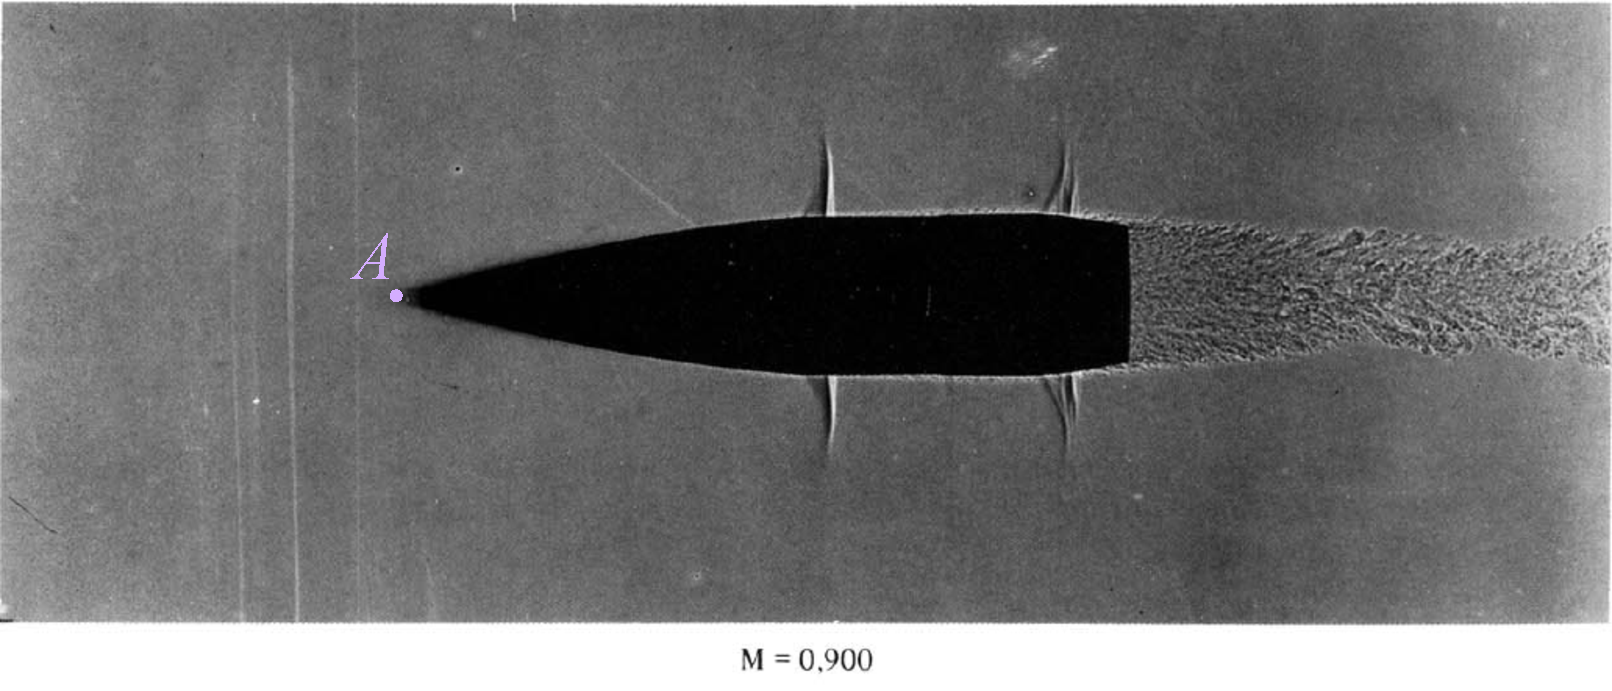
\includegraphics[width=0.7\linewidth]{../img/bullet.pdf}
	
	\parbox{\textwidth}{
	Температура потока в точке торможения $A$ на рисунке вычисляется по формуле
	\[
	T^*  =  
	T \left(
	1 + \displaystyle\frac{\gamma-1}{2} M^2
	\right).
	\]
	Для воздуха ($\gamma \approx 1,4$) при температуре вдали от тела $T=250$~K:
	\begin{enum} %[partopsep=1pt,label=\textbullet]
		\item при $M = 1$ $T^* \approx 290$~K;
		\item при $M = 3$ $T^* \approx 700$~K;
		\item при $M = 5$ $T^* \approx 1500$~K.
	\end{enum}
	
	
	}
	
}

\frame{
	\frametitle{Влияние сжимаемости }

	\parbox{\textwidth}{
		Интегралы Бернулли для давления для несжимаемой жидкости и адиабатического движения газа:
		\[
		p = p^* - \rho_0\frac{v^2}{2}\quad\text{и}\quad
		p = p^*\left(
		1 - \frac{v^2}{v_{max}^2}
		\right)^{\gamma/(\gamma-1)}.
		\]
		
		\vspace{-0.5cm}
		Разложим интеграл для газа в ряд Тейлора по параметру $\displaystyle\frac{v^2}{v_{max}^2} \ll 1$:
		
		\only<1>{
		\[
		p =
		p^*\left(
		1 - \frac{v^2}{v_{max}^2}
		\right)^{\gamma/(\gamma-1)} = 
		\]
		\[
		=
		p^*\left[
		1 - \frac{\gamma}{\gamma-1}\frac{v^2}{v_{max}^2}+ 
		\frac{\frac{\gamma}{\gamma-1}\left(\frac{\gamma}{\gamma-1}-1\right)}{2!}\frac{v^4}{v_{max}^4} + \ldots
		\right] = 
		\]
		
		\centering
		вспомним, что $v_{max}^2 = \displaystyle\frac{2c^{*2}}{\gamma-1}$ и $\displaystyle\frac{\gamma p^*}{\rho^*} = c^{*2}$, тогда
		}
		
		\only<2>
		{
		\[
		=
		p^* - \frac{\rho^*v^2}{2}\left(
		1 - \frac{1}{2(\gamma-1)} \frac{v^2}{v_{max}^2}+ \ldots
		\right)=
%		\]
%		\[
%		=
		p^* - \frac{\rho^*v^2}{2}\left(
		1 - 
		\boxed{\frac{v^2}{4 c^{*2}}} + 
		\ldots
		\right).
		\]
		
%		Отличие двух интегралов в слагаемом $\rho^*v^4/(8c^{*2})$.
		
		Разница не будет превышать $1$~\%, когда
		\[
		 \boxed{v^2/(4c^{*2})} \leq 0,01 \quad\text{или}\quad v \leq c^*/5.
		\]
		При $c^* = 340$~м/с получается условие для скорости $v \leq 68$~м/с.
		}
	

			
	}

	
	
}


\frame{
	\frametitle{Влияние сжимаемости}
	
	
	\parbox{\textwidth}{
	Разложение интеграла Бернулли для плотности по формуле Тейлора имеет вид
	\[
	\frac{\rho}{\rho^*} = 1 - \frac{1}{\gamma-1} \frac{v^2}{v_{max}^2} + \ldots
	\]
	
	Легко проверить, что при $v < \displaystyle\frac{c^*}{5} = 68$~$\displaystyle\frac{\text{м}}{\text{c}}$ будет справедливо
	\[
	\frac{|\rho - \rho^*|}{\rho^*} \leq 0,02.
	\]
		
	}
	
}

\frame{
	\frametitle{ Литература }
	\begin{literature} %[partopsep=1pt,label=\textbullet]
			\item {\em Ван-Дайк М.} Альбом течений жидкости и газа. М.: Мир, 1986.
			
			\item {\em Седов Л.\,И.} Механика сплошной среды. Том 2. М.: Наука, 1970.
	\end{literature}
}

\end{document}
